\documentclass[english]{article}
\usepackage[T1]{fontenc}
\usepackage[latin9]{inputenc}
\usepackage{float}
\usepackage{textcomp}
\usepackage{amsmath}
\usepackage{graphicx}

\makeatletter

\providecommand{\tabularnewline}{\\}

\usepackage{algorithm,algpseudocode}

\makeatother

\usepackage{babel}
\begin{document}

\title{MDPs and TD}

\author{Ajinkya Ambatwar\\
EE16B104\\
Dept. Of Electrical Engineering}
\maketitle
\begin{enumerate}
\item The MDP for the given problem is as follows-\\
\begin{figure}[H]
\includegraphics[angle=90,origin=c,scale=0.3]{Q1_image}\caption{MDP for given table}
\end{figure}
\\
So from the definition of batch MC the value function is as follows-
\begin{align*}
V_{MC}(A) & =1*\frac{2}{3}+2*\frac{1}{3}=\frac{4}{3}\\
V_{MC}(B) & =4/5\\
V_{MC}(C) & =3/5
\end{align*}
\\
For the batch-TD(0) update
\begin{align*}
V_{TD}(B) & =(3/5+0)=0.6\\
V_{TD}(C) & =(4/5+0)=0.8\\
V_{TD}(A) & =\frac{1}{3}(0+0.6)+\frac{2}{3}(0.5+0.8)=16/15
\end{align*}
\\
The MSE values
\begin{align*}
MSE(TD) & =\frac{1}{3}(\frac{16}{15}-\frac{4}{3})^{2}+\frac{1}{5}(0.6-0.6)^{2}+\frac{1}{5}(0.8-0.8)^{2}=0.023\\
MSE(MC) & =\frac{1}{3}(\frac{4}{3}-\frac{4}{3})^{2}+\frac{1}{5}(0.6-0.6)^{2}+\frac{1}{5}(0.8-0.8)^{2}=0
\end{align*}
\\
For training data MC is better as it finds a solution that gives minimum
error on training data. For the model, the TD method gives a better
value as it finds the maximum likelihood estimate of $V^{\pi}$which
also has the highest probabilty of generating data. Hence the error
on future data is minimum for TD estimate given the process in Markov
and hence this estimate is also called as certainty-equivalence estimate.
\item The time index will be taken t mod $\tau$.\\
Hence the monte carlo return- 
\[
G_{t}=R_{(t+1)\%\tau}+\gamma R_{(t+1)\%\tau}....
\]
\\
Similarly the TD(0) update can be given as -
\[
V(S_{t\%\tau})=V(S_{t\%\tau})+\alpha[R_{(t+1)\%\tau}+\gamma V(S_{(t+1)\%\tau})-V(S_{t\%\tau})]
\]
\item For given 3-step eligibility trace truncation, the $\grave{\lambda-return}$
is defined as
\[
G_{t:t+3}^{\lambda}=\hat{v}(S_{t},w_{t-1})+\sum_{i=t}^{t+2}(\gamma\lambda)^{i-t}\delta_{i}^{'}
\]
\\
where $\delta_{i}^{'}=R_{t+1}+\gamma\hat{v}(S_{t+1},w_{t})-\hat{v}(S_{t},w_{t-1})$\\
For general $n$ the expression is as follows-
\[
G_{t:t+n}^{\lambda}=\hat{v}(S_{t},w_{t-1})+\sum_{i=t}^{t+n-1}(\gamma\lambda)^{i-t}\delta_{i}^{'}
\]
\item One of the major reason for Non-Markov model is due to Active Perception.
Active perception refers to the idea that an intelligent agent should
actively control its sensors in order to sense and represent only
the information that is relevant to its immediate ongoing activity.
Tasks that involve active perception lead naturally to non-markov
decision problems since improper control of the sensors leads to internal
representation that fail to encode into relevant to decision making.\\
In such case, a state in the internal representation maps to two or
more states in the external markov model of the system. In such cases,
the markov model of the system based learning methods can not find
a reliable estimate for $V^{\pi}(S)$ for such perpetually aliased
states.\\
This leads to localization errors in the policy function. Use of TD
methods in such case spreads the estimation erros throughout the state
space, thus infecting even policy action for non-aliased states.
\begin{figure}
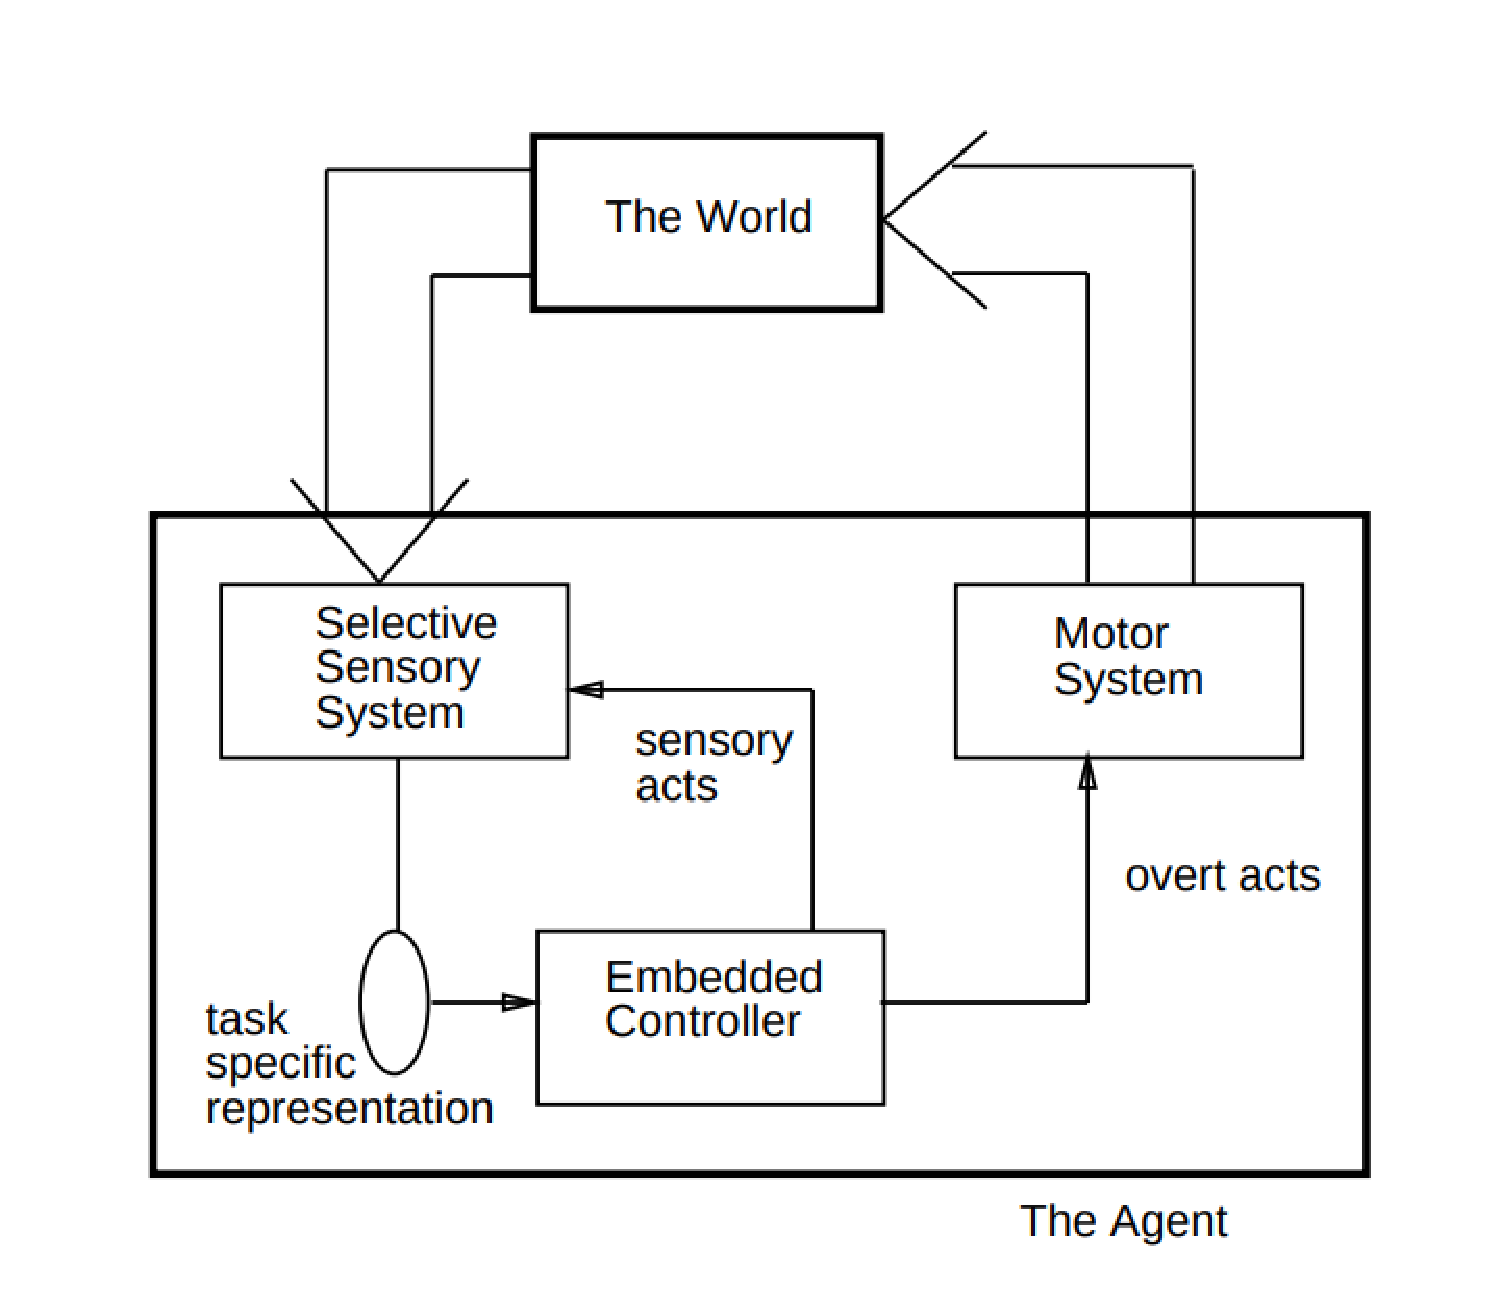
\includegraphics[scale=0.5]{nonmarkov}

\caption{Active Perception model}
\end{figure}
\\
\footnote{Ref: Reinforcement Learning in Non-Markov Environments(Whitehead and
co.,1992)}
\item The grid world is as follows-
\begin{figure}
\includegraphics[scale=0.25]{gridworld}

\caption{Gridworld and Tree Diagram}
\end{figure}
\\
\begin{tabular}{|c|c|c|c||c|c|c}
\hline 
$\pi$ & $S_{1}$ & $S_{2}$ & $S_{3}$ & $V_{1}$ & $V_{2}$ & $V_{3}$\tabularnewline
\hline 
\hline 
1 & Left & - & Left & $a+10\gamma$ & 0 & 10\tabularnewline
\hline 
2 & Left & - & Right & $a+a\gamma+a\gamma^{2}+...$ & 0 & $a+a\gamma+a\gamma^{2}...$\tabularnewline
\hline 
3 & Right & Left & - & 0 & 0 & 0\tabularnewline
\hline 
4 & Right & Right & - & $0+5\gamma$ & $5\gamma$ & 0\tabularnewline
\hline 
5 & Up & - & - & 0 & 0 & 0\tabularnewline
\hline 
\end{tabular}\\
\\
\\
\\
\\
\begin{tabular}{|c|c|c|c|c||c}
\hline 
V & $\pi(1)$ & $\pi(2)$ & $\pi(3)$ & $\pi(4)$ & $\pi(5)$\tabularnewline
\hline 
\hline 
$V_{1}$ & $a+10\gamma$ & $\frac{a}{1-\gamma}$ & 0 & $5\gamma$ & 0\tabularnewline
\hline 
$V_{2}$ & 0 & 0 & 0 & $5\gamma$ & 0\tabularnewline
\hline 
$V_{3}$ & 10 & $\frac{a}{1-\gamma}$ & 0 & 0 & 0\tabularnewline
\hline 
\end{tabular}\\
\\
For calculation of $\pi(S)$ for various values of a and $\gamma$,
let's take an example for $S_{1}$\\
\begin{enumerate}
\item $\pi(S_{1})=\pi(1)$\\
\begin{align*}
a+10\gamma & >\frac{a}{1-\gamma}\\
a+10\gamma & >5\gamma
\end{align*}
\\
The given region can be found out as\\
\begin{figure}[H]

\includegraphics[scale=0.15]{download}
\end{figure}
\\
The solution for this set of inequalities is the region of intersection
shown in the graph. The solution is
\begin{align}
\pi(S_{1}) & =\pi(1)\label{-5<a<0;1>gamma>-a/5}\\
\label{10>a>0;1-(a/10)>gamma>0}
\end{align}
\\
SImilarly we can solve for all other policies for all other states.
The required condition is that
\[
\pi(S_{i})=\pi(j)
\]
\\
when $V_{i}$ corresponding to $\pi(j)$ is highest among values correspondings
all the $\pi(j)$s.
\end{enumerate}
\item In this case we will define a new constant system dynamics $p_{new}(S'|S,a)$
which is not equal to zero for all \{S,A,S'\} pair. The new formulation
for $V^{\pi}$in that case will b\linebreak{}
\begin{align*}
V^{\pi}(s) & =\sum_{s}\pi(a|s)\sum_{s'}\{\frac{p(s'|s,a)}{p_{new}(s'|s,a)}[R(s,a,s')+\gamma v^{\pi}(s')]p_{new}(s'|s,a)\}\\
\end{align*}
\\
So here instead of $p$ the expectation is taken wrt $p_{new}$ and
is of $\frac{p}{p_{new}}(R+\gamma V^{\pi}(s'))$\\
In this way we can get rid of the changing system dynamics and make
it markov. The only condition on $p_{new}$ is that is should be non-zero
for all possible s,a,s' pairs and hence the MDP should have a non-zero
probable transitions from every state to every other state.
\item The on-policy version on Q-learning can be represented as-\\
\begin{enumerate}
\item Choose A from S using policy derived from Q
\item Take action A, observe R,S'
\item Choose A' from S' using policy derived from Q
\item $Q(S,A)=Q(S,A)+\alpha[R+\gamma Q(S',A')-Q(S,A)]$
\item $S=S',A=A'$\\
This way we take action by policy $\pi$ and also be change $\pi$
toward greediness wrt $q_{\pi}$\\
This will converge if all the state-action pairs are met often.
\end{enumerate}
\item The MDP looks like this\\
\includegraphics[angle=180,origin=c,scale=0.3]{noisy}\\
The state set is \{S,L\} (representing Silence and Loudness respectively),
Action set: \{O \ensuremath{\bigwedge} I, O \ensuremath{\bigwedge}
\textlnot I, \textlnot O \ensuremath{\bigwedge} I, \textlnot O \ensuremath{\bigwedge}
\textlnot I\}, where O corresponds to playing the organ, and I corresponds
to burning incense).\\
Using policy iteration as the initial state is Laughing and initial
action is (incense, no organ), there will be no change in the state
as can be seen from the MDP.
\end{enumerate}

\end{document}
